\change{\section{(M3) Short evaluation}}
\label{evaluation}

\change{Before we preceed to our findings on correlations between user mobility and mobile data access patterns, we perform a short evaluation of our speed estimation algorithm in this section. Since the ground truth of user mobility of our dataset is not available to us, we use a similar but much smaller dataset ~\cite{intel-placelab-20041217} collected by Intel Placelab to perform a the evaluation of our speed estimation algorithm. This small dataset contains both cell phone data and GPS traces. We use the GPS as ground truth for the evaluation.}

\change{\subsection{Dataset and Experiment Settings}}

\change{The dataset we used was collected in Seattle area in September 2004. Both cell phone data and GPS data were collected with a Nokia 6600 cell phone and a separate GPS unit. Similar to our dataset, the cell phone data contains only the ID of the cell tower. Note that as the dataset is collected more than ten years ago, so we can only find coordinations for part of the tower IDs contains in the dataset. We thus discarded part of the datasets that contains tower IDs with unknown coordinates. The data we used in our evaluation contains several trips with a total length of 40 minutes and 2007 records.}

\change{We use the same parameter setting as latter we use in our dataset analysis. Thresholds of both distance ratio $d_{ratio}$ and duration ratio $\Delta t_{ratio}$ are ste as 0.6. We are able to get speed estimation for 1955 records out of the total 2007 records. After the filtering, we have 571 that meet both criteria. We also disable both distance lower bound filter and travel time filter by setting thresholds to 0 and use the raw speed estimates as our baseline for comparison. Note that, as we previously stated, if more information such as the underlying road networks are provided, our distance and travel time filters can also be applied to the road trajectories that has the maximum likelihood to match visited tower sequences instead of the straight line trajectories.}

\change{\subsection{Speed estimation accuracy}}

\begin{figure}[h]
    \centering
    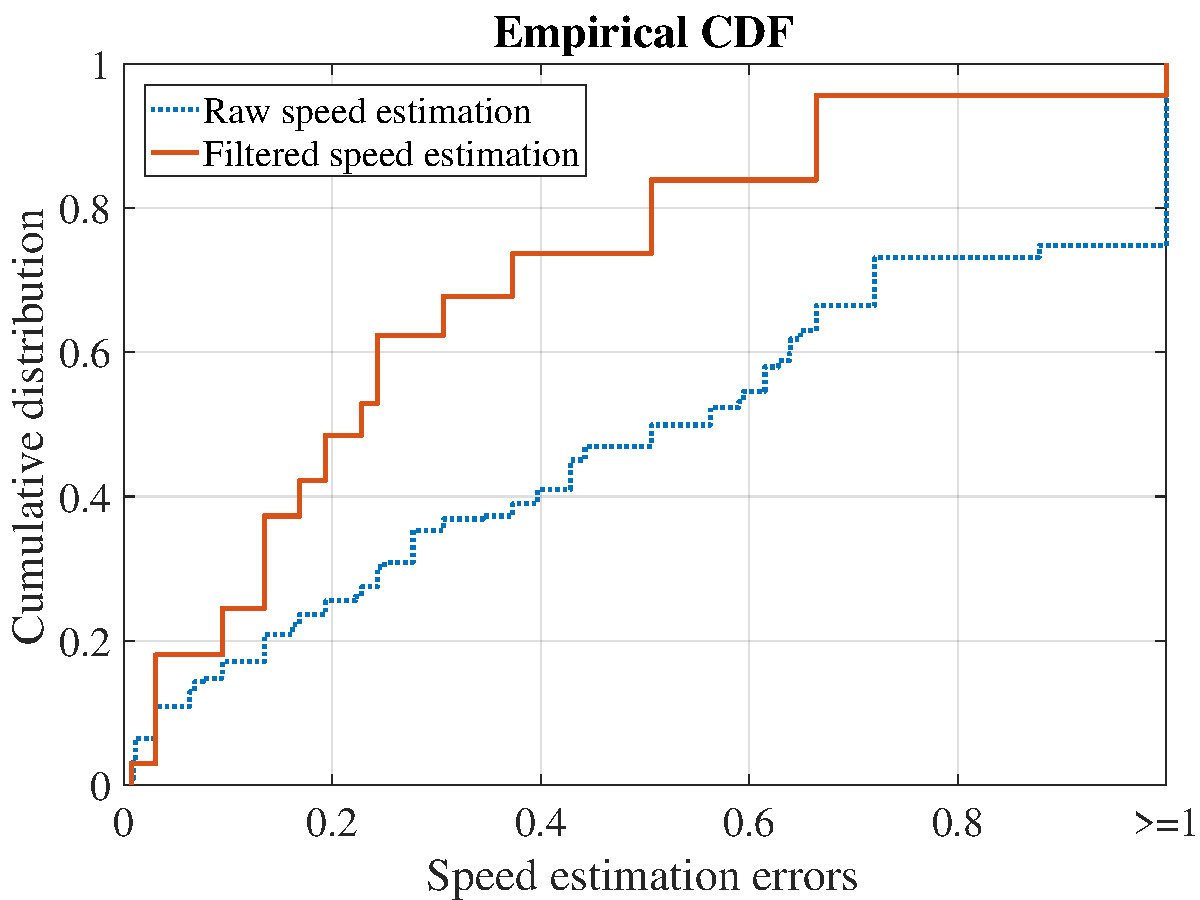
\includegraphics[width=0.5\linewidth]{./figures/cdf_limited.pdf}
    \caption{The CDF of raw speed estimation and filtered speed estimation}
    \label{fig:cdf_limited}
\end{figure}

\change{\autoref{fig:cdf_limited} shows the cdf of errors for both filtered speed estimates and raw speed estimates. Here we define the speed estimation errors as $e = |(s_{est} - s_{gt})| / s_{gt}$, where $s_{est}$ is speed estimated by cell phone data and $s_{gt}$ is ground truth speed calculated by GPS data. By using the absolute value, $e$ is always a positive value. As the value of $e$ can reach to as high as a few hundreds due to cell oscillation problem, we set the limit of $e$ to $1$ in \autoref{fig:cdf_limited} to better show the difference of speed estimation errors in reasonable error range.}

\change{As we can see in \autoref{fig:cdf_limited}, filtered speed estimation significantly outperforms raw speed estimation in terms of accuracy. About 50\% of the filtered speed estimates have less than 0.2 error rate while only 25\% of raw speed estimates achieve the same level of accuracy. More than 80\% of filtered speed estimates have error rates less or equal to 0.5, while for raw speed estimates this number is only less than 50\%. For the high error rate part, there is only less than 5\% of filtered speed estimates have higher than 1 error rates compared to more than 15\% of raw speed estimates have such high error rates.}

\change{\subsection{Speed filtering}}

\begin{figure}[h]
    \centering
    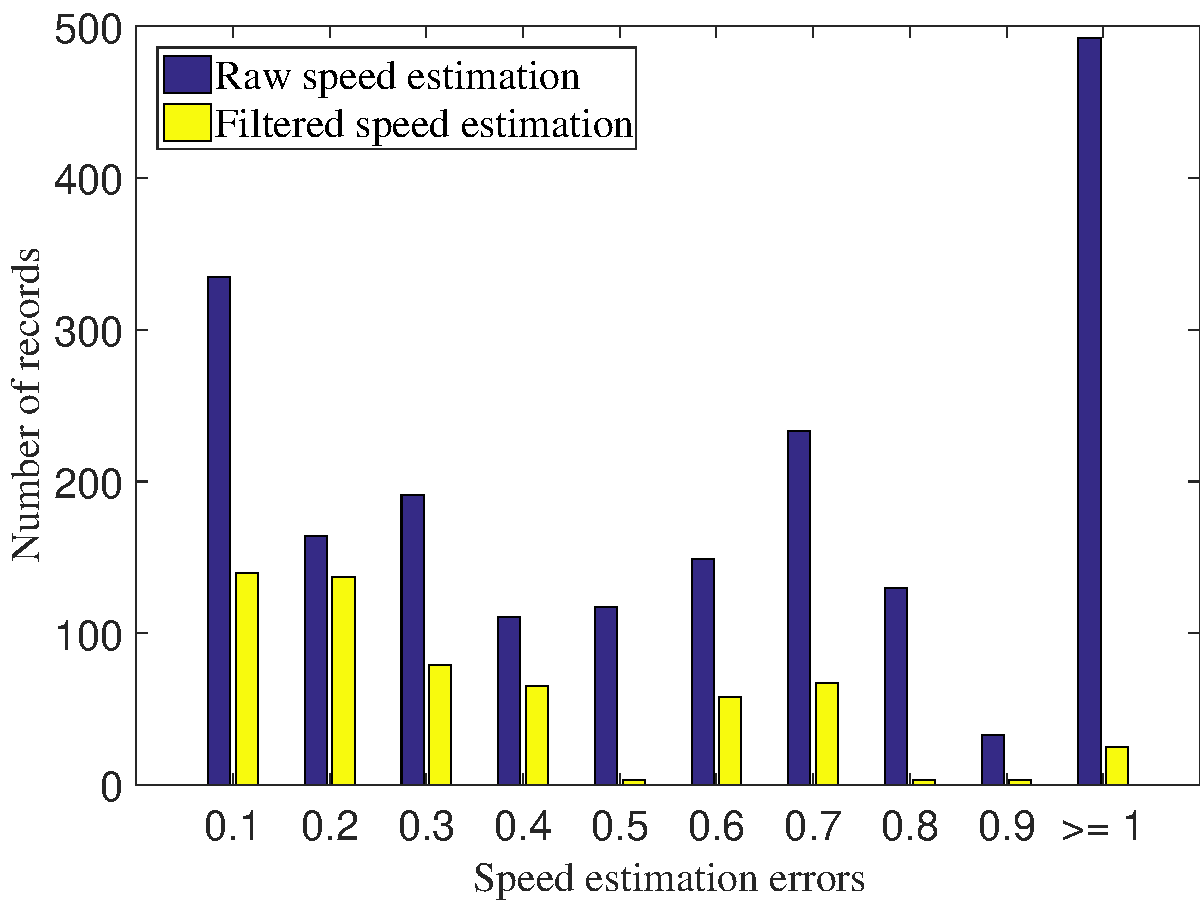
\includegraphics[width=0.5\linewidth]{./figures/error_bar.pdf}
    \caption{Number of records in each error bracket for raw speed estimation and filtered speed estimation}
    \label{fig:error_bar}
\end{figure}

\change{\autoref{fig:error_bar} shows the number of records in each speed estimation error bracket. For example, there are around 350 data records have raw speed estimates with an error rate of 0.1. Among these 350 data records, only around 150 data records have filtered speed estimates. The rest 200 data records are filtered our by our speed estimation algorithm. Is worth noting that our speed estimation algorithm does not improve speed estimation accuracy on a single data record. Actually, it filtered out those speed estimates that have possible high error rates by setting up threshold for both distance and travel time. In \autoref{fig:error_bar}, we can see that approximately 50\% of records that have raw speed estimation errors less than 0.5 have been filtered out while more than 85\% of records that have raw speed estimation errors greater than 0.5 have been filtered out.}